\section{Design}\label{sec:design}
% section outcomes
This section provides the overall architecture of our project and discusses the main design choices that we made.

An understanding of the existing Colladoc architecture was necessary to ensure that the system implemented would fit seamlessly into the existing product. 
Many of the design decisions that we made were influenced by the fact that Colladoc Smart Search is an extension to Colladoc.
Fig. \ref{fig:product-design} shows the original Colladoc architecture in italic and Colladoc Smart Search extensions in bold. 
\begin{figure}[h!t]
\begin{center}
\leavevmode
{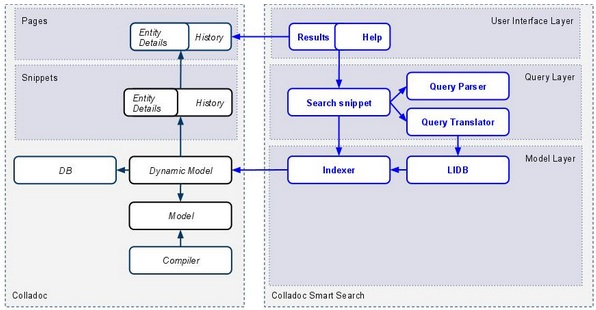
\includegraphics[width=0.9\textwidth]{design}}
\end{center}
\caption{Product Design}
\label{fig:product-design}
\end{figure}
Colladoc uses the Scala compiler front-end to create a documentation model (or just Model) from the source code input. This documentation model is used to provide the symbol information and code documentation that is visualised in Colladoc. Wiki-like editing of documentation is achieved by extending the original model to a Dynamic Model, which allows documentation changes. Changes for each documentation symbol are persisted in a database. “Snippets”
generate dynamic content based on the information provided by the Model. Pages visualize this content.

The overall design of Colladoc Smart Search separates the system into layers. We defined three layers of Colladoc Smart Search  - Model, Query and UI layers. 

The \textbf{Model layer} contains components which access the documentation model, analyze it and add it to a search index database. ${SearchIndexer}$ is the main component in that layer.

The \textbf{Query layer} contains components which take search queries,  execute them and return the result. When the user enters a search query string, the $SearchSnippet$ passes it to a $QueryParser$ that generates an abstract representation of the query. The search-engine independent representation is transformed by Query Transformer to specific query objects used by the search engine. The $SearchSnippet$ generates the search result content and passes it to the UI layer.

The \textbf{UI layer} contains components which present the search results to the user.